\section{Theorie}
\label{sec:Theorie}
In der Thermodynamik wird jeder räumlich abgegrenzte Bereich, in dem ein Stoff
sich in einem homogenen Zustand befindet, als Phase bezeichnet, beispielsweise
die Aggregatszustände fest, flüssig und gasförmig. Durch Änderung des Drucks oder
der Temperatur des Stoffes, kann ein Übergang von einer Phase in eine andere
Phase auftreten. Mit den Bedingungen, wann ein solcher Phasenübergang auftritt,
lassen sich in einem Zustands- oder Phasendiagramm, in welchem der Druck $p$
gegen die Temperatur $T$ aufgetragen ist, drei Bereiche abgrenzen. Diese sind in
der Abbildung \ref{fig:phasendiagramm} zu sehen.
\begin{figure}[H]
  \centering
  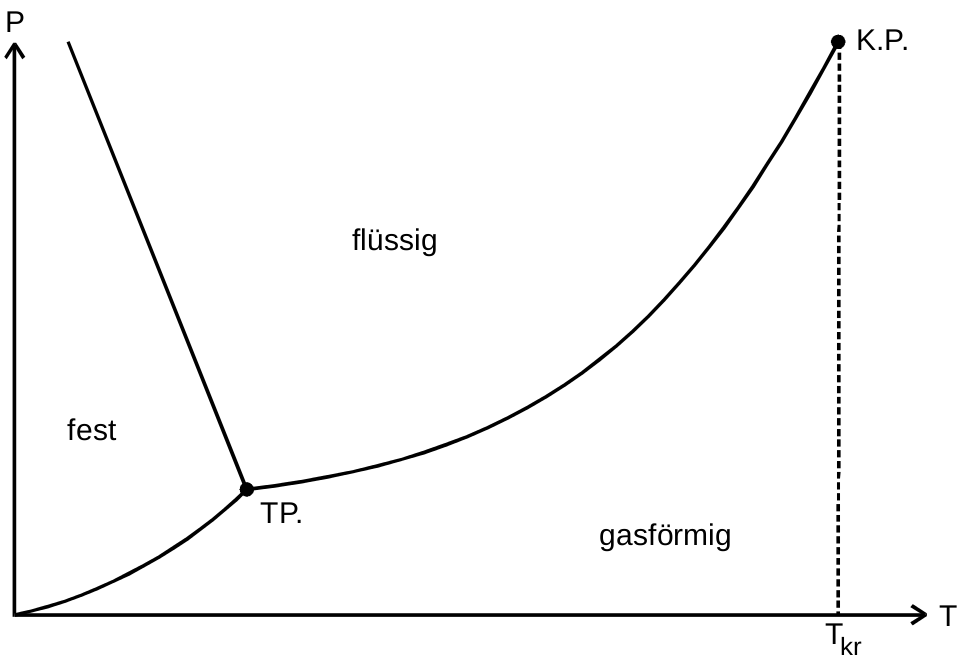
\includegraphics[width=0.7\textwidth]{phasendiagramm.png}
  \caption{qualitatives Phasendiagramm des Wassers \cite{sample}.}
  \label{fig:phasendiagramm}
\end{figure}
\noindent Innerhalb eines jeden Bereiches besitzt das System zwei Freiheitsgrade, das heißt,
dass das Wasser jeden Wert für den Druck $p$ oder die Temperatur $T$, der innerhalb
einer Kurve liegt, annehmen kann, ohne in eine andere Phase überzugehen. Entlang
jeder der abgrenzenden Kurven besitzt das System nur noch einen Freiheitsgrad.
Wenn die Temperatur vorgegeben ist, ist der Druck durch die Kurve vorgegeben.

In dem Phasendiagramm sind zwei besondere Punkte markiert: der kritische Punkt
(K.P.) und der Tripelpunkt (TP). Im kritischen Punkt koexistieren die flüssige
und die gasförmige Phase, im Tripelpunkt koexistieren alle drei Phasen nebeneinander
und sind nicht mehr unterscheidbar.

Zwischen dem Tripelpunkt und dem kritischen Punkt liegt die Dampfdruckkurve, als
Übergang von der flüssigen zur gasförmigen Phase. Der Verlauf der Dampfdruckkurve
ist sehr stark abhängig von der Verdampfungswärme $L$, welche eine temperaturabhängige
Materialeigenschaft ist. Nahe bei dem Tripelpunkt ist die Verdampfungswärme
ungefähr konstant, in der Nähe des kritischen Punktes geht sie gegen Null.

Die molare Verdampfungswärme bezeichnet die Energie, welche zur Umwandlung von
einem Mol einer Flüssigkeit in Dampf bei gleichbleibender Temperatur benötig wird.
Jedem Molekül ist nach der Maxwellschen Geschwindigkeitsverteilung eine
Geschwindigkeit zugeordnet. Die Moleküle mit maximaler kinetischer Energie können
die Molekularkräfte überwinden und die Flüssigkeit verlassen. Dadurch erhöht die
Anzahl der Gasmoleküle, welche somit mehr Stöße auf die Wand des Gefäßes ausüben
und den Druck erhöhen. Bei Stößen mit der Flüssigkeitsoberfläche können jedoch
auch Moleküle wieder in die Flüssigkeit eintauchen. Mit der Zeit stellt sich
ein Gleichgewichtszustand mit einem konstanten Sättigungsdampfdruck ein.

Aus einem reversiblen Kreisprozess, wie er in Abbildung \ref{fig:kreisprozess}
dargestellt ist, bei dem zunächst isotherm und isobar ein Mol eines Stoffes
verdampft und anschließend wieder kondensiert wird, lässt sich unter
Berücksichtigung der zugführten mechanischen Energie, die zum Verdampfen nötig ist,
die Clausius-Clapeyronsche Differentialgleichung
\begin{equation}
  (V_\text{D} - V_\text{F}) \symup{d}p = \frac{L}{T}\symup{d}T
  \label{eqn:clausius}
\end{equation}
aufstellen. Dabei ist $V_\text{D}$ das Volumen des Dampfes, $V_\text{F}$ das
Volumen der Flüssigkeit, $L$ die Verdampfungswärme und $T$ die Temperatur.
\begin{figure}
  \centering
  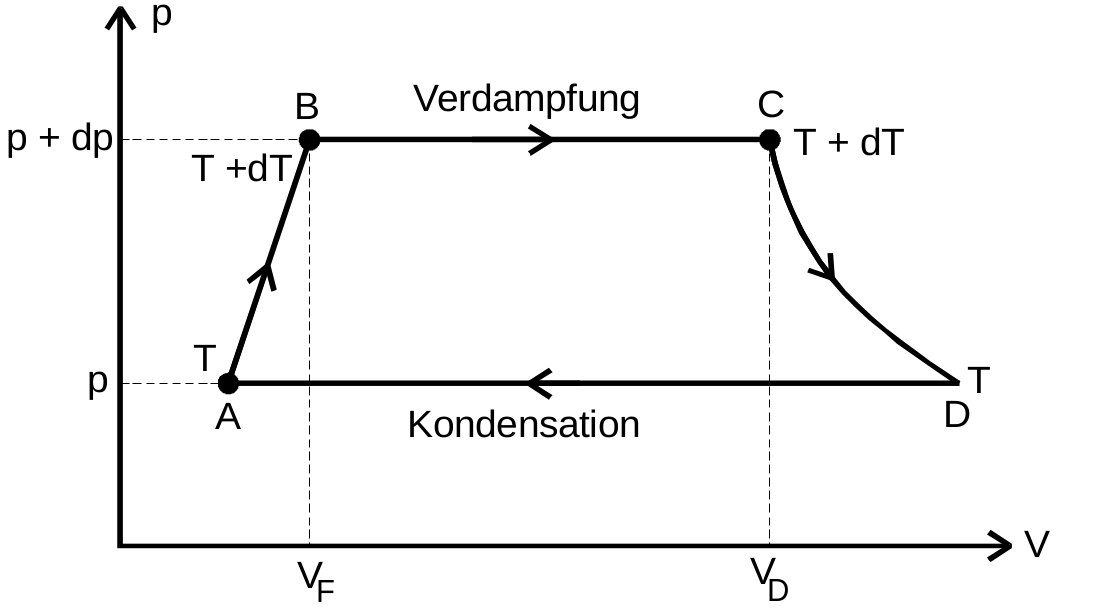
\includegraphics[width=0.7\textwidth]{kreisprozess.png}
  \caption{Reversibler Kreisprozess, bei dem die Flüssigkeit zunächst erwärmt und
  dann Verdampft wird und danach wieder abgekühlt wird und Kondensiert \cite{sample}.}
  \label{fig:kreisprozess}
\end{figure}
Da die Integration dieser Differentialgleichung im Allgemeinen schwierig
ist, werden folgende vereinfachenden Näherungen angenommen:
\begin{enumerate}
  \item Das Volumen $V_\text{F}$ der Flüssigkeit ist gegenüber dem Volumen $V_\text{D}$
  des Dampfes vernachlässigbar,
  \item Das Dampfvolumen $V_\text{D}$ verhält sich nach der idealen Glasgleichung
  \begin{equation}
    V_\text{D}(p,T) = R \frac{T}{p}
    \label{eqn:ideale_Gasgleichung}
  \end{equation}
  und
  \item Die Verdampfungswärme $L$ ist temperaturunabhängig.
\end{enumerate}
Damit hat die Clausius-Clapeyronsche Differentialgleichung \eqref{eqn:clausius}
die neue Form
\begin{equation}
  \frac{R}{p}\symup{d}p = \frac{L}{T^2}\symup{d}{T},
  \label{eqn:clausius_vereinfacht}
\end{equation}
mit dem Druck $p$ und der allgemeinen Gaskonstante $R=\SI{8.3142}{\joule\per\mol\kelvin}$.
Diese wird durch
\begin{equation}
  p = p_0 e^{-\frac{L}{R T}}
  \label{eqn:loesung_dgl}
\end{equation}
gelöst. \cite{sample}
